% status: 100
% chapter: IaaS

\title{Google Compute Engine}


\author{Bertolt Sobolik}
\orcid{1234-5678-9012}
\affiliation{%
  \institution{Indiana University}
  \city{Bloomington} 
  \state{Indiana} 
  \postcode{47408}
}
\email{bsobolik@iu.edu}

% The default list of authors is too long for headers}
\renewcommand{\shortauthors}{B. Sobolik}


\begin{abstract}
Google Compute Engine is an Infrastructure as a Service (IaaS)
offering from Google. The company offers a wide variety of virtual
machines, operating systems, and storage options to serve a wide
variety of customers, including many high-end options and
configurations designed for specific applications. The history of the
offering is described as well as the expansion of locations. Details
about the types of virtual machines, images, and additional hardware
available are provided. Advanced features like live migration and
preemtible VMs are discussed. An overview of the competitve landscape
is presented to put Google's offering into the context of the overall
IaaS marketplace.
\end{abstract}

\keywords{hid-sp18-419, E519, Google, Compute, Engine}


\maketitle

\section{Introduction}
Compute Engine is Google's Infrastructure as a Service (IaaS)
offering. IaaS is ``a standardized, highly automated offering, where
compute resources, complemented by storage and networking capabilities
are owned and hosted by a service provider and offered to customers
on-demand~\cite{hid-sp18-419-gartneritglossaryiaas}.''  Customers run
virtual machines for which they choose the operating system and
storage, but they do not have control over the underlying hardware or
network infrastructure~\cite{hid-sp18-419-mell2011nist}. IaaS
providers generally differentiate themselves based on pricing, service
level agreements (SLA), storage and networking options, and the types
of database and application development services that they
offer~\cite{hid-sp18-419-perficientchoosingiaas}. Google attempts to
further distinguish their IaaS offering from the offerings of their
competitors with claims of environmental friendliness and greater
flexibility manifest in the availibility of \textit{Preemtible
Instances}, which are VMs that automatically terminate after 24 hours
or if resources are needed for other purposes. Preemptible instances
are offered at a lower cost than other VMs. They are useful for batch
processing jobs or other situations where VMs are needed for
activities that are fault-tolerant and not time
sensitive~\cite{hid-sp18-419-gce}.


\section{History}
A preview edition of Google Compute Engine was launched on June 28,
2012~\cite{hid-sp18-419-googleblog20120628} to expand on the
capabilities of Google App Engine, which had been around since
2008~\cite{hid-sp18-419-gcp-history-medium}. The preview release
supported Debian and Centos linux distributions that Google had
customized to some extent. Google Compute Engine was made an official
Google product on December 2, 2013. When it became an official product
support was added for SELinux, CoreOS, SUSE, FreeBSD, and other Linux
distributions. Support was also added for Docker, FOG, xfs, and
aufs. Early customers included Snapchat and
Evite~\cite{hid-sp18-419-googleblog20131202}. The first Google
platform Live event was held in San Francisco on March 25, 2014. At
the second such event on November
4~\cite{hid-sp18-419-googleblog20140812}, 2014 Google announced the
release of Compute Engine Autoscaler which allows developers to
dynamically resize VMs in response to utilization or other triggers,
and the beta release of Local SSD, allowing users to attach local
solid-state drive block storage to VM instances. Some technology
journalists saw this event and its many announcements, including the
launch of Google Container Engine, Google Cloud Interconnect (which
allowed customers to connect directly to Google's data
centers~\cite{hid-sp18-419-gcp-techcrunch-20141104}), and many
enhancements to Google App Engine, as a sign that Google was getting
more serious about competing with Amazon in the cloud computing
market~\cite{hid-sp18-419-forbes-gcp-20141104}.

In January, 2015, Local SSD became generally available, and Google
Cloud Monitoring, including support for Compute Engine went into
beta~\cite{hid-sp18-419-googleblog20150113}. These enhancements were
made possible as a result of the integration of Stackdriver, which
Google acquired in May of
2014~\cite{hid-sp18-419-googleblog20140507}. The beta release of
Preemptible Instances happend in May, 2015 followed by the official
release in September of the same
year~\cite{hid-sp18-419-venturebeat-preemptive-vms}. Citadel and
Descartes Labs were early adopters of the
technology~\cite{hid-sp18-419-googleblog20150518}. In July, 2015
Google added Windows Server to the VMs available on Compute
Engine~\cite{hid-sp18-419-googleblog20150715}, which had been in beta
since December, 2014~\cite{hid-sp18-419-googleblog20141208}. This
enabled them to compete more effectively with Microsoft Azure IaaS,
which at the time was much closer to Amazon EC2 in overall IaaS market
share than it is today~\cite{hid-sp18-419-statista-iaas-market2015}.

The beta release of Nvidia Tesla K80 GPUs on Google Compute Engine was
announced in February of 2017, allowing customers to attach up to
eight GPUs to a custom VM. At the same time, Intel Skylake processors
were made available in a number of
regions~\cite{hid-sp18-419-googleblog20170221}.

In March, 2017 Google enhanced their support of Microsoft SQL Server
on GCP, adding SQL Server Enterprise images to the VMs available along
with a number of other relational database
announcements~\cite{hid-sp18-419-googleblog20170309}.

In May of 2017, Google expanded their machine types available as
Compute Engine VMs, offering VMs with up to 64 virtual processors and
up to 416 GB of memory which are certified for running SAP's in-memory
database HANA. In October, 2017 Google increased their top offering to
96 CPUs and 624 GB of memory, and they are reported to be working on
products that will deliver 4 TB of
memory~\cite{hid-sp18-419-techcrunch-gce-20171005}.

In February, 2018 Google added the ability to create VMs from
templates based on existing VM
instances~\cite{hid-sp18-419-googleblog20180222}.

\section{Locations}
One thing that made it difficult for Google to compete effectively
with other players in the IaaS space was how few regional data centers
the company had relative to their competitors. From the beta launch of
the service in 2012 until mid-2014, they only had two locations,
us-central1 in Iowa and europe-west1 in
Belgium~\cite{hid-sp18-419-gcp-history-medium}. Expansion to the
Asia-Pacific region was announced on April 14, 2014 with the openning
of asia-east1 in Taiwan to support customers in the region including
Applibot, an mobile gaming company in Japan, and Tagtoo, an content
tagging startup in Taiwan. Japanese and Traditional Chinese language
web sites and developer consoles were launched at the same
time~\cite{hid-sp18-419-googleblog20140414}. They started offering
services to GCP customers from an additional sites, us-east1 in South
Carolina, in October, 2015. Before this the site had only been used
for Google's internal applications. At the time us-east1 was launched
Microsoft had 20 locations hosting Azure
services~\cite{hid-sp18-419-techcrunch-gcp-20151001}. Another
location, us-west1 in Oregon was made available to GCP customers in
July, 2016, and a Tokyo location was announced in March, 2016 and went
live in November 2016~\cite{hid-sp18-419-googleblog20161108}. The
Oregon location was seen as critical to making their service
attractive to the online gaming community. They anticipated a 30-80\%
reduction in latency for customers located in cities on the west coast
of the US with the launch of
us-west1~\cite{hid-sp18-419-googleblog20160720}.

In September, 2016 Google announced eight additional
locations~\cite{hid-sp18-419-gcp-history-medium}:
\begin{itemize}
  \item Mumbai
  \item Singapore
  \item Sydney
  \item Northern Virginia (launched May 2017)
  \item São Paulo
  \item London (launched July 2017)
  \item Finland
  \item Frankfurt
\end{itemize}

Currently, Google has 15 locations on five contenents: five in North
America, four in Europe, four in Asia, and one each in South America
and Australia. Each region is broken out into two to four
zones. Certain resources are only available in certain zones within a
location, and some resources must be in the same zone. For example, a
disk must be in the same zone as the instance to which it is attached,
and GPUs are only available in certain zones within certain
regions~\cite{hid-sp18-419-gce-regions-zones}.


\section{Virtual Machine Types}

Google offers 25 different standard machine types. Machine types are
defined by the number of virtual CPUs, gigabytes of memory, maximum
number of persistent disks, and the maximum total size of persistent
disk storage available. The two smallest instances, f1-micro and
g1-small, respectively run on .2 and .5 fractions of a shared physical
core and have .6 or 1.7 GB of memory. These VMs are limited to 4
persistent disks totaling 3 terrabytes. The other 23 machine types are
named with the prefix n1. Customers can choose from five different
Intel Xeon E5 processors for these instances ranging from the the
older 2.6 GHz Sandy Bridge to the fifth-generation 2.0 GHz
Skylake. Depending on the region and zone of the VM certain processors
and configurations are not available.

The \textit{n1-} prefix VMs are organized into three groups: standard,
high-memory, and high-cpu. There is a single CPU option for the
standard configuration, which has 3.75 GB of memory. The other 22
options are configured with two to 96 CPUs, and differ from each other
by the amount of memory offered, ranging from 1.8GB for the
n1-highcpu-2 configuration to 1.4TB for the n1-megamem-96. Up to 16
persistant disks adding up to a total of 16 TB of persistent storage
can be attached to any of the n1 prefixed VMs, which can be augmented
with additional storage from Google Cloud Platform's variety of
database and blob storage options. Custom machine types are also
available, and up to 128 persistent disks can be attached in beta VM
configurations~\cite{hid-sp18-419-gce-machine-types}.

Configurations of VMs can be saved in instances templates and
organized in groups for easier scaling and overall management. Managed
instance groups can automatically scale, perform load balancing, and
automatically recreate unhealthy or failed instances within the
group. Managed instance groups can be within one zone or in multiple
zones in a single region~\cite{hid-sp18-419-gce-instance-groups}.

\section{Additional Hardware}

Graphics Processing Units (GPUs) can be attached to VMs configured
with one to 64 Broadwell (fourth generation) Xeon E5 CPUs. NVIDIA
Tesla K80 GPUs are generally available. NVIDIA Tesla P100 GPUs are
available in beta only, which means that they are not covered under
any SLA. VMs with K80 GPUs are not coverd by SLAs in certain zones as
well. GPUs are only available on VMs in certain zones, all of which
are located in the US, Europe, and Asia. Customers can attach up to
eight K80 GPUs or up to four P100 GPUs, which can be configured with
one to 416 GB of memory, depending on the zone, the number and the
type of GPUs attached. Also available in beta is the ability to create
preemptible instances with GPUs attached to
them~\cite{hid-sp18-419-gce-gpus}.

Google's custom-developed application-specific integrated circuits
(ASICs), dubbed Tensor Processing Units (TPUs), can also be attached
to VMs for accellerating machine learning applications using
TensorFlow, an open source machine learning software library developed
by Google~\cite{hid-sp18-419-tensorflow}. They are marketed under a
separate brand ``Cloud TPU'' and are only released in
beta~\cite{hid-sp18-419-cloud-tpu}.

\section{Images}
Google allows a wide variety of images to run on Compute Engine
VMs. The company provides public images for several versions of linux,
including CentOS and Ubuntu. Premium images include RedHat Enterprise
and several versions of Windows Server. Google also offers images for
specific application, including the company's own container-optimized
OS, VMs designed to run SAP, and SQL Server on Windows Server. With
the exception of Google's container-optimized OS, these special
purpose images are all priced at the company's premium tier.

Google also allows custom images to run on Compute Engine VMs, as well
as a few community-supported images: Debian Testing, openSUSE, and
FreeBSD. Customers running custom images can save them so that they
can be easily redeployed on a number of different VM
instances. Multiple releases are available for most
images~\cite{hid-sp18-419-gce-images}.


\section{Live Migration}
Google provides customers with the ability to keep instances up and
running seemlessly through maintainence, certain hardware failures,
upgrades, and some configuration changes through a technology they
call \textit{Live Migration}. The components
involved in making live migration work is shown in
Figure~\ref{f:live-migration}.

\begin{figure}[!ht]
  \centering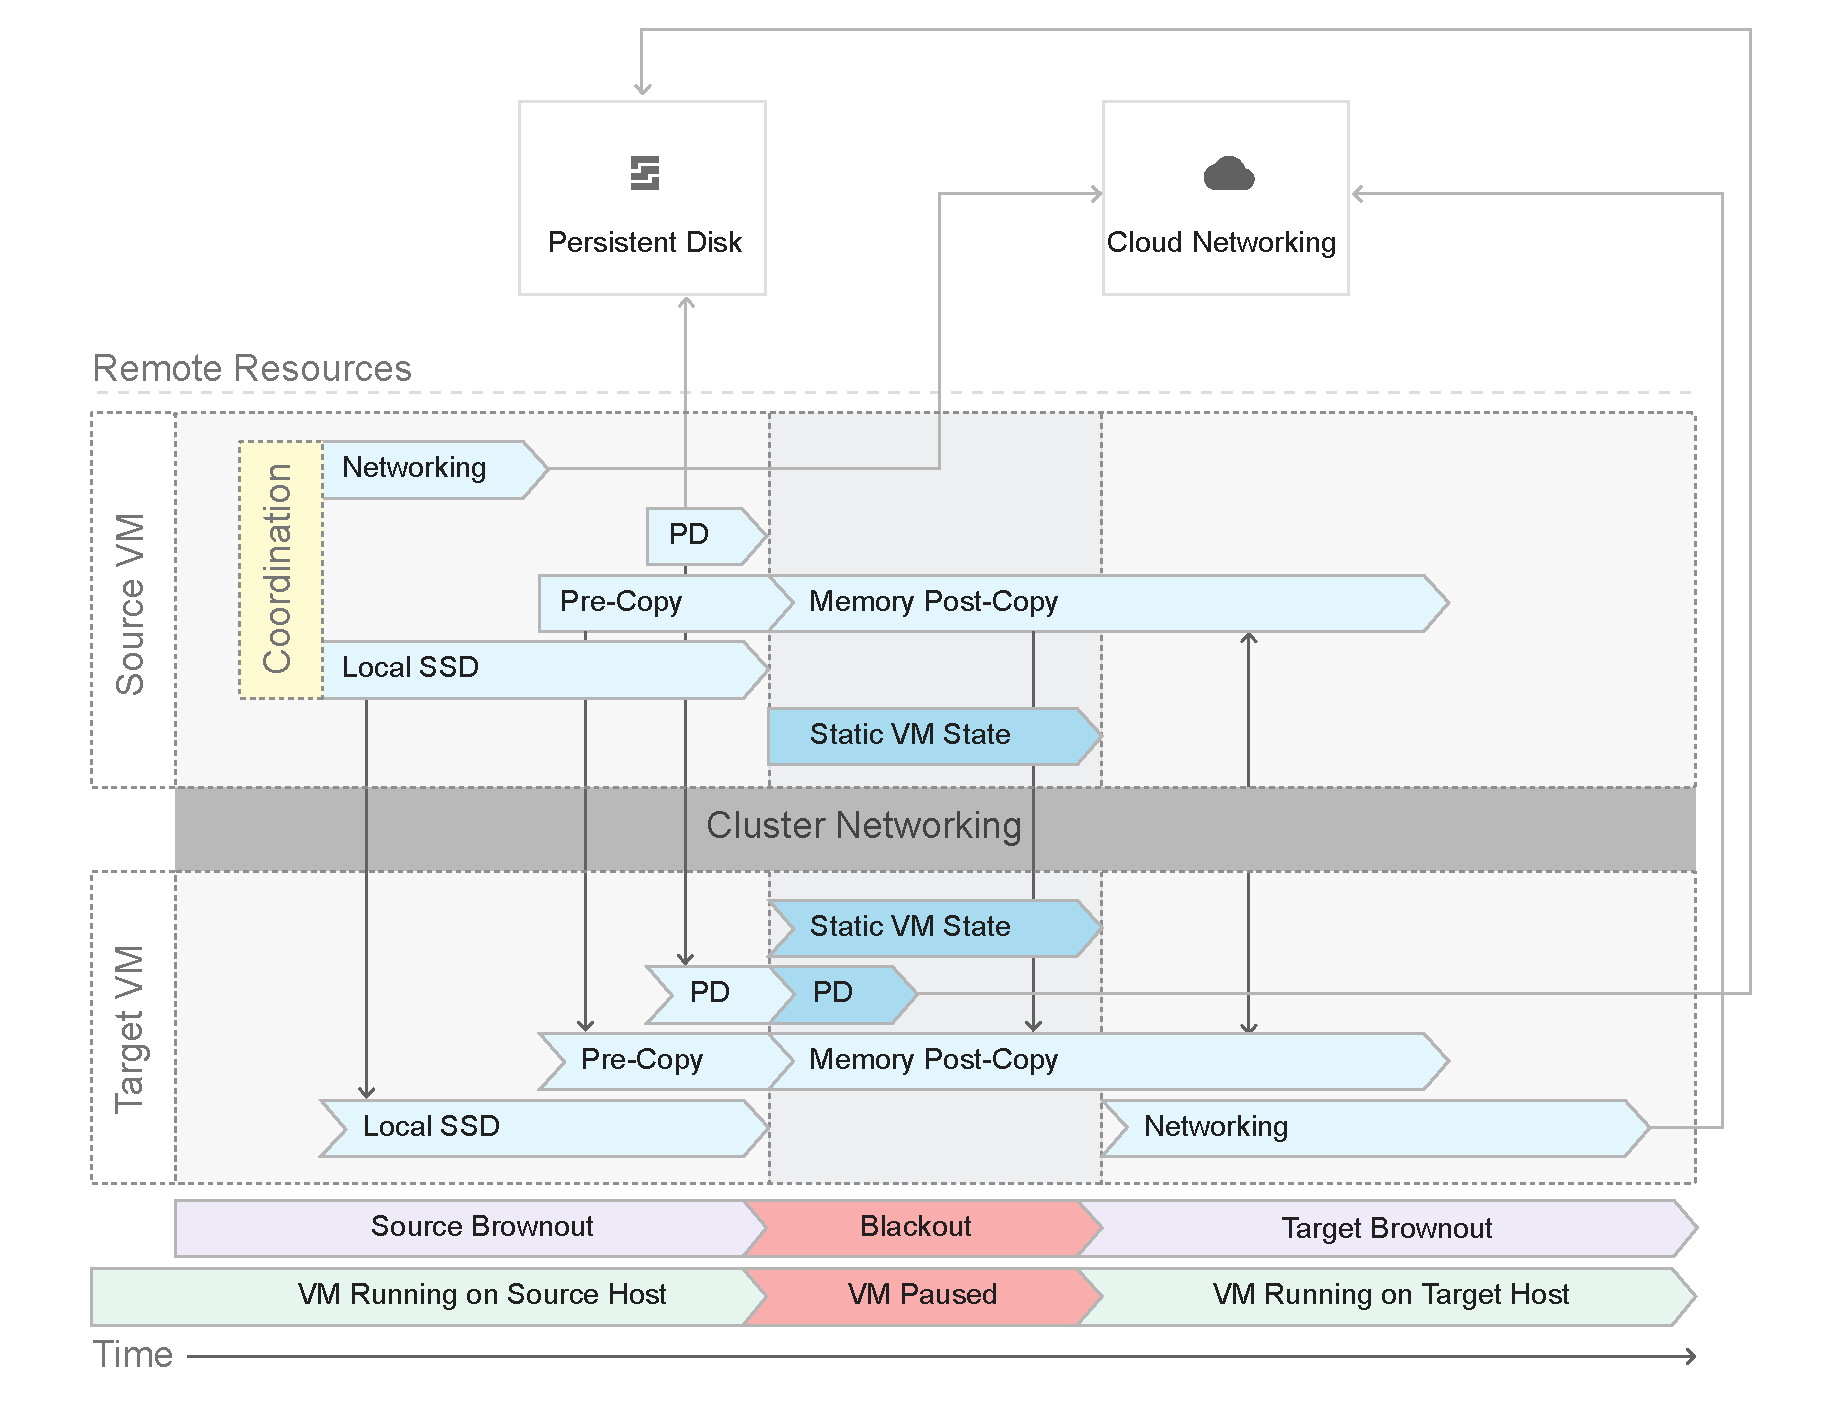
\includegraphics[width=\columnwidth]{images/live-migration.pdf}
  \caption{Google Compute Engine live migration components~\cite{hid-sp18-419-gce-live-migration}}\label{f:live-migration}
\end{figure}

Live migration is not an option for VMs
with GPUs attached or for preemptible
instances~\cite{hid-sp18-419-gce-live-migration}.

\section{Competitors and Market Share}

Google Compute Engine's main competitors are Amazon Elastic Cloud
Compute (EC2), Microsoft Azure IaaS, AlibabaCloud Elastic Compute
Service, and Rackspace Public Cloud. Amazon is by far the leader in
this space with 44.2\% of total revenue in 2016 (almost \$10
billion). In terms of revenue, Google Compute Engine was the fourth
largest IaaS public cloud service, behind Amazon, Microsoft, and
Alibaba but ahead of Rackspace due to year over year growth from
2015. In 2016, GCP's revenue doubled from \$250 million in 2015
to \$500 million. GCP had a 2.3\% share of the IaaS market in 2016 and
is growing faster than all of the above named competitors except for
Alibaba, which grew 126.5\% in 2016~\cite{hid-sp18-419-gartnerpr2017}.


\section{Conclusion}

Google arrived into the IaaS market later than some more successful
competitors. The company has recently made some very significant
investments in features and infrastructure. They have attempted to
differentiate themselves from their competitors with headline-grabbing
massive instances and high-end add-ons like GPUs and TPUs. They also
have attempted to appeal to budget-minded customers with services like
preembtible VMs and to the environmentally conscious with greener data
centers.

The company's offering in the IaaS space is designed to appeal to a
wide variety of customers and it will be interesting to see how it
continues to evolve over time.


\begin{acks}

  The authors would like to thank Dr.~Gregor~von~Laszewski for his
  support and suggestions to write this paper.

\end{acks}

\bibliographystyle{ACM-Reference-Format}
\bibliography{report} 

